\documentclass[12pt,oneside]{article}
%Per attivare / disattivare le soluzioni andare in 
%setting.tex e modificare il campo typeSol 
%   • S = "show" mostra le soluzioni
%   • H = "Hide/Show" mostra le soluzioni quando premute
%   • N = "Not" Non mostrare le soluzioni

%TODO: Riuscire a correggere il fatto che premendo su una si mostrino tutte le soluzioni in un colpo solo, creare quindi frame distinti ogni volta 
% Author: Izaak Neutelings (March 2020)
\usepackage{color}
\definecolor{editorGray}{rgb}{0.95, 0.95, 0.95}
\definecolor{editorOcher}{rgb}{1, 0.5, 0} % #FF7F00 -> rgb(239, 169, 0)
\definecolor{editorGreen}{rgb}{0, 0.5, 0} % #007C00 -> rgb(0, 124, 0)
\usepackage{upquote}
\usepackage{listings}
\lstdefinelanguage{JavaScript}{
  morekeywords={typeof, new, true, false, catch, function, return, null, catch, switch, var, if, in, while, do, else, case, break},
  morecomment=[s]{/*}{*/},
  morecomment=[l]//,
  morestring=[b]",
  morestring=[b]'
}

\lstdefinelanguage{HTML5}{
        language=html,
        sensitive=true, 
        alsoletter={<>=-},
        otherkeywords={
        % HTML tags
        <html>, <head>, <title>, </title>, <meta, />, </head>, <body>,
        <canvas, \/canvas>, <script>, </script>, </body>, </html>, <!, html>, <style>, </style>, ><
        },  
        ndkeywords={
        % General
        =,
        % HTML attributes
        charset=, id=, width=, height=,
        % CSS properties
        border:, transform:, -moz-transform:, transition-duration:, transition-property:, transition-timing-function:
        },  
        morecomment=[s]{<!--}{-->},
        tag=[s]
}

\lstset{%
    % Basic design
    backgroundcolor=\color{editorGray},
    basicstyle={\small\ttfamily},   
    frame=l,
    % Line numbers
    xleftmargin={0.75cm},
    numbers=left,
    stepnumber=1,
    firstnumber=1,
    numberfirstline=true,
    % Code design   
    keywordstyle=\color{blue}\bfseries,
    commentstyle=\color{darkgray}\ttfamily,
    ndkeywordstyle=\color{editorGreen}\bfseries,
    stringstyle=\color{editorOcher},
    % Code
    language=HTML5,
    alsolanguage=JavaScript,
    alsodigit={.:;},
    tabsize=2,
    showtabs=false,
    showspaces=false,
    showstringspaces=false,
    extendedchars=true,
    breaklines=true,        
    % Support for German umlauts
    literate=%
    {Ö}{{\"O}}1
    {Ä}{{\"A}}1
    {Ü}{{\"U}}1
    {ß}{{\ss}}1
    {ü}{{\"u}}1
    {ä}{{\"a}}1
    {ö}{{\"o}}1
}


\usepackage{amsmath} % for \dfrac
\usepackage{physics}
\usepackage{tikz,pgfplots}
\usepackage{tikz-3dplot}
\usepackage[outline]{contour} % glow around text
\usetikzlibrary{angles,quotes} % for pic (angle labels)
\usetikzlibrary{arrows,arrows.meta}
\usetikzlibrary{calc}
\usetikzlibrary{decorations.markings}
\tikzset{>=latex} % for LaTeX arrow head
\usepackage{xcolor}
\colorlet{Ecol}{orange!90!black}
\colorlet{EcolFL}{orange!90!black}
\colorlet{veccol}{green!45!black}
\colorlet{Bcol}{violet!90}
\colorlet{Bcol1}{violet!80!blue!90}
\colorlet{Bcol2}{violet!80!red!90}
\colorlet{BFcol}{red!60!black}
\colorlet{veccol}{green!45!black}
\colorlet{Icol}{blue!70!black}
\tikzstyle{BField}=[->,thick,Bcol]
\tikzstyle{current}=[->,Icol,thick]
\tikzstyle{force}=[->,thick,BFcol]
\tikzstyle{vector}=[->,thick,veccol]
\colorlet{pluscol}{red!60!black}
\colorlet{minuscol}{blue!60!black}
\tikzstyle{charge+}=[very thin,draw=black,top color=red!50,bottom color=red!90!black,shading angle=20,circle,inner sep=0.3]
\tikzstyle{charge-}=[very thin,draw=black,top color=blue!50,bottom color=blue!80,shading angle=20,circle,inner sep=0.3]
\tikzstyle{metal}=[top color=black!15,bottom color=black!25,middle color=black!20,shading angle=10]
\tikzstyle{light metal}=[top color=black!10,bottom color=black!15,middle color=black!6,shading angle=10]
\tikzset{
  EFieldLine/.style={thick,EcolFL,decoration={markings,mark=at position #1 with {\arrow{latex}}},
                     postaction={decorate}},
  EFieldLine/.default=0.5,
  BFieldLine/.style={thick,Bcol,decoration={markings,mark=at position #1 with {\arrow{latex}}},
                                 postaction={decorate}},
  BFieldLine/.default=0.5,
  pics/Bin/.style={
    code={
      \def\R{0.12}
      \draw[pic actions,line width=0.6,#1,fill=white] % ,thick
        (0,0) circle (\R) (-135:.75*\R) -- (45:.75*\R) (-45:.75*\R) -- (135:.75*\R);
  }},
  pics/Bout/.style={
    code={
      \def\R{0.12}
      \draw[pic actions,line width=0.6,#1,fill=white] (0,0) circle (\R);
      \fill[pic actions,#1] (0,0) circle (0.3*\R);
  }},
  pics/Bin/.default=Bcol,
  pics/Bout/.default=Bcol,
  pics/magnet/.style={ %args={#1}
    code={
      \def\h{0.9}
      \coordinate (-N) at (0,\h);
      \coordinate (-S) at (0,-\h);
      \draw[pic actions,thick,top color=red!60,bottom color=red!90,shading angle=20]
        (-0.8*\h/2,0) rectangle ++(0.8*\h,\h);
      \draw[pic actions,thick,top color=blue!60,bottom color=blue!90,shading angle=20]
        (-0.8*\h/2,0) rectangle ++(0.8*\h,-\h);
      \node[pic actions] at (0, \h/2) {\textbf{N}};
      \node[pic actions] at (0,-\h/2) {\textbf{S}};
  }},
}
\tikzstyle{measure}=[<->,fill=white,midway,outer sep=0]
\contourlength{1.5pt}

\tikzset{
    my dotted/.style={dash pattern=on 0pt off 4pt, line cap=round},
    my dashed/.style={dash pattern=on 3pt off 3pt}, 
    mydashdotted/.style={dash pattern=on 3pt off 3pt on 0pt off 3pt, line cap=round}
}

\usepackage{pythonhighlight}
\usepackage[Glenn]{fncychap}
%\usepackage[italian]{babel}
\usepackage{hhline}
\usepackage{pdfpages}
\usepackage{fontspec}
\newcommand{\mymk}[1]{%
  \tikz[baseline=(char.base)]\node[anchor=south west, draw,rectangle, rounded corners, inner sep=2pt, minimum size=7mm,
    text height=2mm](char){\ensuremath{#1}} ;}

\newcommand*\circled[1]{\tikz[baseline=(char.base)]{
            \node[shape=circle,draw,inner sep=2pt,anchor = base] (char) {#1};}}
%\setmainfont{Times new Roman}
\usepackage{geometry}
\newcommand{\centered}[1]{\begin{tabular}{l} #1 \end{tabular}}
\usepackage{pgfplots}
\usepackage{caption}
\usepackage{multicol}
\usepackage{xcolor}
\usepackage{erewhon}
\usepackage{marginnote}
\usepackage{lettrine}
\usepackage{wrapfig}
\usepackage{lipsum}
\usepackage{GoudyIn}
\usepackage{yfonts,color}
\usepackage{amssymb}
\usepackage{amsmath}
\usepackage{dsfont}
\usepackage[many]{tcolorbox}
\usepackage{multicol}
\usepackage{pdfpages}
\usepackage{circuitikz}
\usepackage{xcolor}
\usepackage{pagecolor}

%\setcounter{DefaultLines}{3}%

\usepackage{tikz,pgfplots}
\usetikzlibrary{intersections}
\pgfplotsset{compat=1.18, width=8cm, height=7cm}
\usepackage{cancel}
\usepackage{fancyhdr}
\usepackage{hhline}
\geometry{
    a4paper,
    total={170mm, 275mm},
    top={20mm},
    bottom={20mm}
}
\usepackage{calligra}
\thispagestyle{empty}


\date{}

\vspace*{2\baselineskip}
\usepackage{hyperref}

\newcommand*{\titleGP}{
    \vspace{-40pt} 
    \begingroup 
    \centering  % Ambiente di centratura
    \vspace*{\baselineskip}
    \rule{\textwidth}{1.6pt}\vspace*{-\baselineskip}\vspace*{2pt}
    \rule{\textwidth}{0.4pt}\\[\baselineskip]
    {\LARGE{Robotics first assignement} \\ 
    \normalsize{\calligra{Matteo Padrin 2199438 }}}\\
    [0.2\baselineskip]
    \\ 
\href{https://github.com/matteopadrin15-beep/RoboticsProject}{%
    \raisebox{-0.3\height}{
\includegraphics[width=0.07\linewidth]{github.png}}%
    \hspace{0.2cm} % Spazio tra icona e link
    \texttt{github.com/matteopadrin15-beep/RoboticsProject}%
}
        \rule{\textwidth}{0.4pt}\vspace*{-\baselineskip}\vspace{3.2pt}
    \rule{\textwidth}{1.6pt}\\[\baselineskip]
    \scshape  % Piccolo maiuscolo
    \endgroup  % Chiudi il gruppo
}
\newcommand*\Eval[3]{\left.#1\right\rvert_{#2}^{#3}}
\DeclareMathOperator{\di}{d\!}
\newcommand{\Lap}{\mathcal{L}}
\newcommand{\fem}{\mathcal{E}}
\newcommand{\D}{\mathbb{D}}
\newcommand{\R}{\mathbb{R}}
\newcommand{\Q}{\mathbb{Q}}
\newcommand{\N}{\mathbb{N}}
\newcommand{\C}{\mathbb{C}}
\newcommand{\Z}{\mathbb{Z}}
\newcommand{\x}{x_0}
\newcommand{\y}{y_0}
\newcommand{\comp}[2]{#1 \circ #2}
\newcommand{\acc}{acc^{ne}}
\newcommand{\Def}{def^{nte}}
\newcommand{\sub}[1]{#1 \subseteq \R }
\newcommand{\Succ}[1]{#1_{n}}
\newcommand{\Lim}[4]{\lim_{#1\to #2} #3\ = #4}
\newcommand{\liminfty}{\lim_{x \to +\infty}}

\newcommand{\der}[1]{#1^{'}}
\newcommand{\dersx}[1]{\der{#1}_{-}}
\newcommand{\derdx}[1]{\der{#1}_{+}}
\newcommand{\dder}[1]{#1^{''}}
\newcommand{\inv}[1]{#1^{-1}}
\newcommand{\T}{T_{n,\x}[}
\newcommand{\Px}[1]{a_{n} #1^{n} + a_{n-1} #1^{n-1} + ... + a_{1} #1+ a_{0}}
\makeatletter
\newcommand*{\rom}[1]{\expandafter\@slowromancap\romannumeral #1@}
\makeatother
\newcommand{\vasymptote}[2][]{
    \draw [densely dashed,#1] ({rel axis cs:0,0} -| {axis cs:#2,0}) -- ({rel axis cs:0,1} -| {axis cs:#2,0});
}

\pgfplotsset{
    double y domain/.code 2 args={
        \pgfmathsetmacro\doubleymin{#1*2}
        \pgfmathsetmacro\doubleymax{#2*2}
    },
    ejes/.style args={#1:#2 #3:#4}{
        double y domain={#3}{#4},
        domain=#1:#2,
        ymin=#3,ymax=#4, restrict y to domain=\doubleymin:\doubleymax,
        samples=100,
        enlargelimits=false,
        axis lines=middle,
        xtick={#1,...,#2}, ytick={#3,...,#4},
        xticklabels=\empty, yticklabels=\empty,
        every axis plot post/.style={
            black,
            mark=none,
            smooth
        },
        scale only axis,
        width=4cm,
        height=4cm
    }
}
\usepackage{colortbl}
\usepackage{steinmetz}
\newenvironment{sistema}% 
{\left\lbrace\begin{array}{@{}l@{}}}% 
{\end{array}\right.}
\usepackage{scrextend,tikz,scalerel}
\renewcommand{\thefootnote}{\roman{footnote}}
\deffootnotemark{\textsuperscript{\vspace{0.1cm}\smash{\circled{\thefootnotemark}}}}
\newcounter{Es}
\newcounter{Hide}
\setcounter{Hide}{0}
\usepackage{ocgx2} %Per attivare / disattivare le soluzioni 
\newcommand\typeSol{S}
\newcommand\Solution[1]
{
    %S means show
    \if \typeSol S {#1} \fi 

    %H means partially hide 
    \if \typeSol H {\switchocg{\theHide \myC}{Premere per mostrare / nascondere la soluzione} 
    \begin{ocg}{My Layer}{\theHide}{off}
    #1
    \end{ocg}
    \addtocounter{Hide}{1}
    }
    \fi

    %N means not shown
    \if \typeSol N {} \fi
}

\definecolor{myYellow}{RGB}{255, 255, 190}
\newcommand{\codice}[1]
{
\colorbox{myYellow}{%
    \parbox{\dimexpr\linewidth-2\fboxsep}{\texttt{#1}}%
}
}


\newcommand{\drawarm}[5]{%
  \coordinate (O)  at (0,0);
  \coordinate (J1) at ([shift={(#1:1)}]O);
  \coordinate (J2) at ([shift={(#2:1)}]J1);
  \coordinate (J3) at ([shift={(#3:1)}]J2);
 
  \draw[gray!40, thin] (-0.4,0) -- (1.8,0);
  \draw[gray!40, thin] (0,-0.4) -- (0,2.6);
 
  \draw[blue!70!black,   line width=2.2pt, line cap=round, #5] (O)  -- (J1);
  \draw[teal!70!black,   line width=2.2pt, line cap=round, #5] (J1) -- (J2);
  \draw[orange!80!black, line width=2.2pt, line cap=round, mydashdotted] (J2) -- (J3);
  
  \filldraw[gray!50]          (O)  circle (1.5pt);
  
  \filldraw[draw=blue!70!black, fill = blue!70!white]    (J1) circle (1.5pt);
  \filldraw[draw=teal!70!black, fill =teal!70!white]    (J2) circle (1.5pt);
  \filldraw[fill=red!70!black]     (J3) circle (2pt);
  \node[right=4pt, font=\small] at (J3) {$(1,\,2)$};
 
  \node[below left, font=\small] at (O) {$O$};
 
  \node[font=\large\bfseries] at (0.7,-0.35) {#4};
}
\newcommand{\myrule}{%
  \vspace{2mm}%
  \hrule%
  \vspace{2mm}%
}
\newcommand{\shortrule}{%
  \vspace{0.5mm}%
  \hrule%
  \vspace{0.5mm}%
}
\usepackage{booktabs}
\usepackage{bm}

\usetikzlibrary{calc,patterns,angles,quotes}
\usepackage{pgfplots}
\usepackage{subfig}
\usepackage{multicol}
\usepackage{float}
\usepackage{tabularx}
\usepackage{tabularx}
\setcounter{Es}{0}

\usepackage{amsthm}

\newcommand{\myhrule}{ \vspace{0.2cm} \hrule \vspace{0.2cm}}
\newcommand\iseq{\stackrel{\mathclap{\mbox{?}}}{=}}
\lstset{
  language=Java,
  basicstyle=\ttfamily\small,
  keywordstyle=\color{blue}\bfseries,
  commentstyle=\color{green!50!black}\itshape,
  stringstyle=\color{red},
  backgroundcolor=\color{gray!10},
  numbers=left,
  numberstyle=\tiny\color{gray},
  stepnumber=1,
  numbersep=5pt,
  showstringspaces=false,
  tabsize=2,
  breaklines=true,
  captionpos=b
}
\newtcolorbox{Es}[2][]{
    colback=blue!10, enhanced, %Grigio
    title= \textbf{#1}, % Autoincrementa e mostra il contatore Es
    attach boxed title to top left={xshift=-4mm},
    boxrule=0pt, after skip=1cm, before skip=1cm, right skip=0cm,
    breakable, fonttitle=\bfseries,
    toprule=0pt, bottomrule=0pt, rightrule=0pt, leftrule=4pt,
    arc=0mm, skin=enhancedlast jigsaw, sharp corners,
    colframe=gree, colbacktitle=gre,
    boxed title style={
        frame code={ 
            \fill[gre](frame.south west)--(frame.north west)--(frame.north east)--
            ([xshift=\the\dimexpr(#2+3mm)]frame.east)--(frame.south east)--cycle;
            \draw[line width=1mm,gre]([xshift=\the\dimexpr(#2+2mm)]frame.north east)--
            ([xshift=\the\dimexpr(#2+5mm)]frame.east)--([xshift=\the\dimexpr(#2+2mm)]frame.south east);
            \draw[line width=1mm,gre]([xshift=\the\dimexpr(#2+5mm)]frame.north east)--
            ([xshift=\the\dimexpr(#2+8mm)]frame.east)--([xshift=\the\dimexpr(#2+5mm)]frame.south east);
            \fill[blue!40](frame.south west)--+(4mm,-2mm)--+(4mm,2mm)--cycle; %Grigio
        }
    }
}
\newtcolorbox[]{examplebox}[2][]{%
  enhanced,                         % abilita codice TikZ interno
  colback=white,                    % colore di sfondo
  colframe=white,                   % colore del bordo
  coltitle=black,                   % colore del titolo
  fonttitle=\bfseries,              % titolo in grassetto
  left=4mm, right=2mm,              % margini interni
  arc=6mm,                          % angoli leggermente arrotondati
  boxrule=0.5pt,                    % spessore del bordo principale
  borderline west={2pt}{-1mm}{black}, % linea verticale a sinistra (leggermente estesa)
  title=\large #2,                  % titolo in grande
  #1
}
\newcommand{\ct}[1]{\texttt{#1}}
%\definecolor{gre}{RGB}{160, 160, 160}
%\definecolor{gree}{RGB}{32, 32, 32}

\definecolor{gree}{RGB}{153, 255, 255}
\definecolor{gre}{RGB}{51, 51, 255}

\definecolor{mGreen}{rgb}{0,0.6,0}
\definecolor{mGray}{rgb}{0.5,0.5,0.5}
\definecolor{mPurple}{rgb}{0.58,0,0.82}
\definecolor{backgroundColour}{rgb}{0.95,0.95,0.92}
\newcommand{\rn}{\textbackslash r \textbackslash n}
\lstdefinestyle{CStyle}{
    backgroundcolor=\color{backgroundColour},   
    commentstyle=\color{mGreen},
    keywordstyle=\color{magenta},
    numberstyle=\tiny\color{mGray},
    stringstyle=\color{mPurple},
    basicstyle=\ttfamily\footnotesize,
    breakatwhitespace=false,         
    breaklines=true,                 
    captionpos=b,                    
    keepspaces=true,                 
    numbers=left,                    
    numbersep=5pt,                  
    showspaces=false,                
    showstringspaces=false,
    showtabs=false,                  
    tabsize=2,
    language=C,
    frame=single,
    breaklines=true,
    breakatwhitespace=true,
    columns=fullflexible
}
\lstdefinestyle{HTMLStyle}{
    language=HTML,
    basicstyle=\ttfamily\small,
    backgroundcolor=\color{gray!10},
    frame=single,
    breaklines=true,
    columns=fullflexible,
    showstringspaces=false,
    captionpos=b
}
\newcommand{\intorno}{\mathcal{I}_\varepsilon}

\newtcolorbox[]{examplebox}[2][]{%
  enhanced,                         % abilita codice TikZ interno
  colback=white,                    % colore di sfondo
  colframe=white,                   % colore del bordo
  coltitle=black,                   % colore del titolo
  fonttitle=\bfseries,              % titolo in grassetto
  left=4mm, right=2mm,              % margini interni
  arc=6mm,                          % angoli leggermente arrotondati
  boxrule=0.5pt,                    % spessore del bordo principale
  borderline west={2pt}{-1mm}{black}, % linea verticale a sinistra (leggermente estesa)
  title=\large #2,                  % titolo in grande
  #1
}
\usepackage[many]{tcolorbox}
\tcbuselibrary{minted}
\tcbset{
texexp/.style={colframe=red!50!yellow!50!black, colback=red!50!yellow!5!white,
coltitle=red!50!yellow!3!white,
fonttitle=\small\sffamily\bfseries, fontupper=\small, fontlower=\small},
example/.style 2 args={texexp,
title={Example \thetcbcounter: #1},label={#2}},
}
\newtcblisting{texexp}[1]{texexp,#1}
\newtcblisting[auto counter,number within=section]{texexptitled}[3][]{%
example={#2}{#3},#1}
\newtcolorbox[use counter from=texexptitled]{texexptitledspec}[3][]{%
example={#2}{#3},#1}




\reversemarginpar
\renewcommand{\contentsname}{Indice}
\newtheorem{thm}{Theorem}%[section]
\begin{document}
\titleGP
\section*{How to run the code}

\subsection*{Dependencies}
All dependencies are installable via \texttt{pip}:
\texttt{pip install numpy sympy matplotlib}
\begin{center}
\begin{tabular}{lll}
\toprule
\textbf{Library} & \textbf{Version tested} & \textbf{Purpose} \\
\midrule
\texttt{numpy}      & $\geq$ 1.24 & Numerical computation, matrix operations \\
\texttt{sympy}      & $\geq$ 1.12 & Symbolic Jacobian computation and lambdification \\
\texttt{matplotlib} & $\geq$ 3.7  & Trajectory plotting \\
\bottomrule
\end{tabular}
\end{center}

\subsection*{How to run the code}
\codice{python robtics.py}

Simply run the code, and it will open all the windows needed for the assignment 
\section*{Part 1}
Since we are dealing with a robotic arm, the angles $\alpha$ and $2\pi+\alpha$ are equivalent in the final position, therefore in this solution we restrict to $\theta_i \in [-\pi,\pi) , i\in \{1,2,3\}$. 

\begin{comment}
\begin{figure}
    \centering
    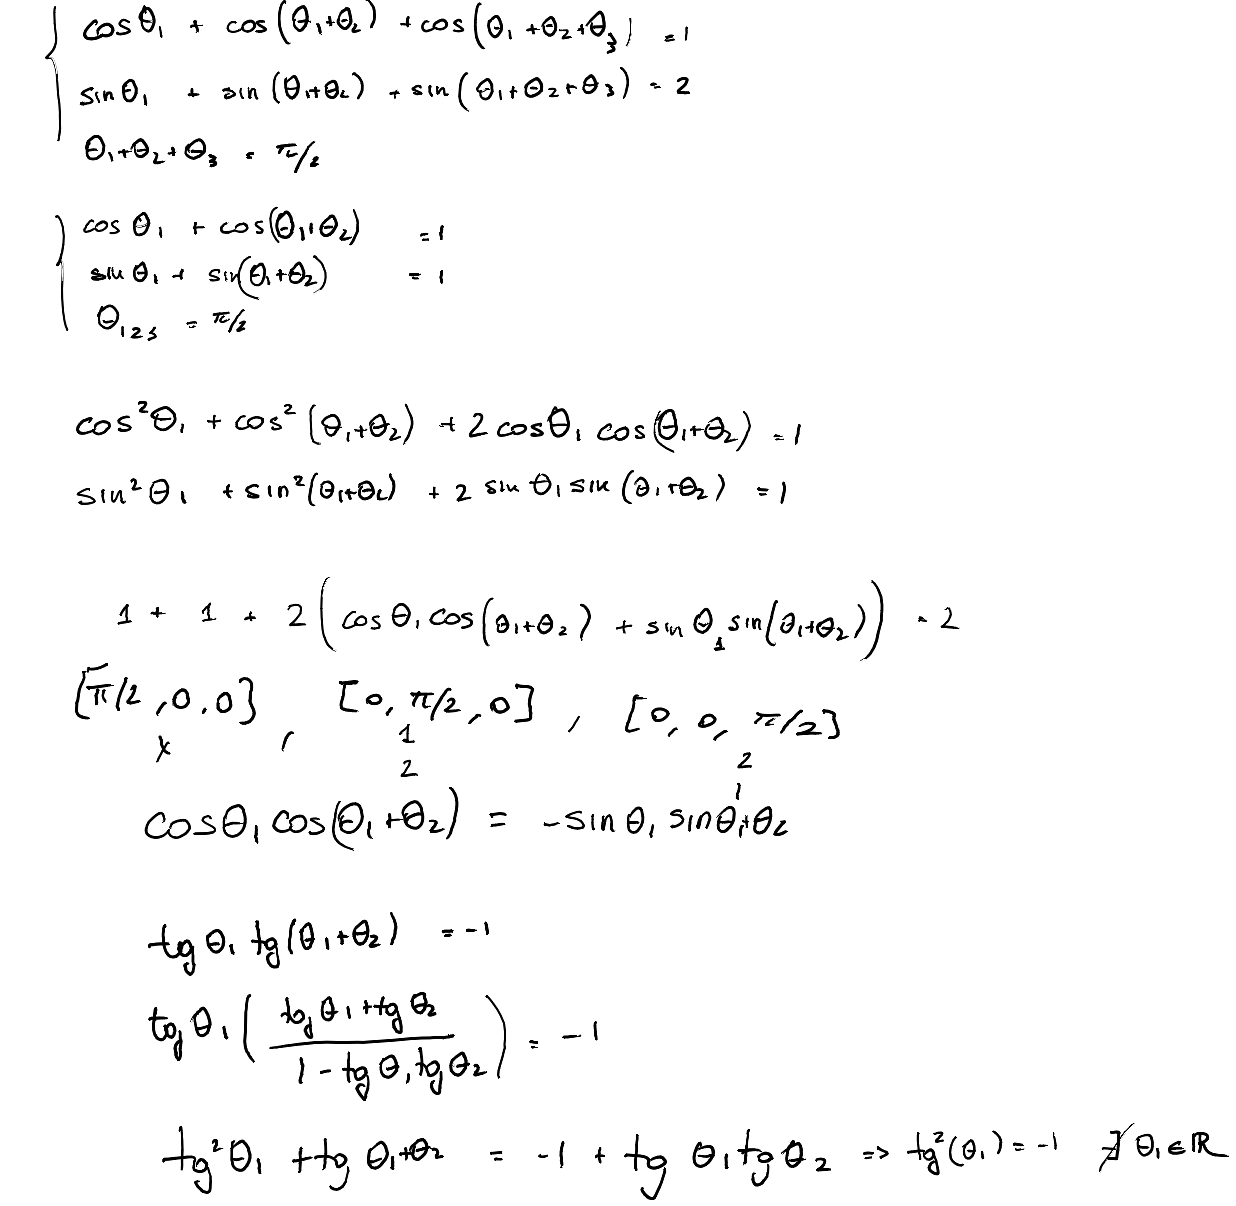
\includegraphics[width=0.5\linewidth]{Base.png}
\end{figure}
\end{comment}


To find the angles $\vec\theta=[\theta_1\, \theta_2 \, \theta_3]^\top$, we need to solve the following system
$$\begin{cases}
    \cos(\theta_1) + \cos(\theta_1+\theta_2) + \cos(\theta_1+\theta_2+\theta_3) = 1 \\ 
    \sin(\theta_1) + \sin(\theta_1+\theta_2) + \sin(\theta_1+\theta_2+\theta_3) = 2\\ 
    \theta_1+\theta_2+\theta_3 = \dfrac{\pi}{2}
\end{cases}$$
Therefore from the last equation, we can simplify the model to 
$$\begin{cases}
    \cos(\theta_1) + \cos(\theta_1+\theta_2)  = 1 \\ 
    \sin(\theta_1) + \sin(\theta_1+\theta_2) +1 = 2\\ 
    \theta_1+\theta_2+\theta_3 = \dfrac{\pi}{2}
\end{cases}$$
By squaring both sides and summing the first two equations, we get 
$$ 1+1+2\bigg(\cos(\theta_1)\cos(\theta_1+\theta_2) + \sin(\theta_1)\sin(\theta_1+\theta_2) \bigg) =2$$
Which implies that 
\begin{equation*}
   \cos(\theta_1)\cos(\theta_1+\theta_2) = - \sin(\theta_1)\sin(\theta_1+\theta_2) \tag{$\star$}
\end{equation*}
This is equivalent to $\tan(\theta_1)\tan(\theta_1+\theta_2) = -1$ only if the two cosines are not equal to zero, therefore there are three (+ 1) subcases starting from $\star$: the first one is if neither of them is different form zero, if $\cos(\theta_1) = 0$ and the other two arise when $\cos(\theta_1+\theta_2) = 0$. 
\begin{comment}
\begin{figure}
    \centering
    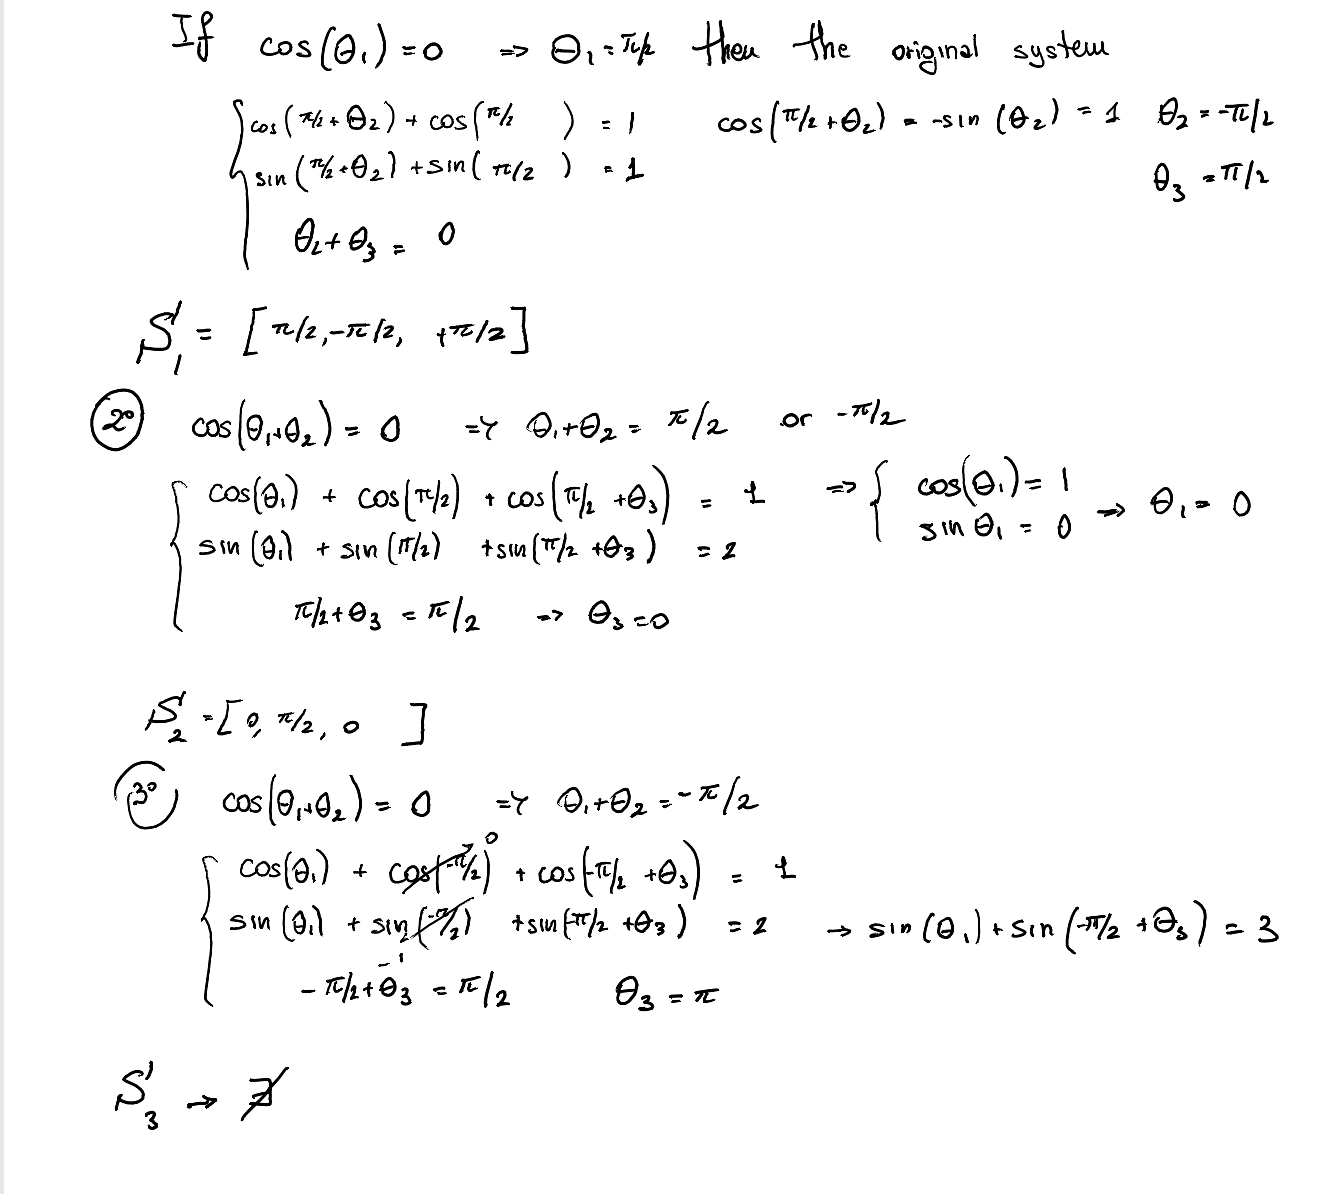
\includegraphics[width=0.5\linewidth]{Casistiche.png}
\end{figure}
\end{comment}
\newpage
\begin{tcolorbox}[title={Case 1: $\cos(\theta_1)=0$}, colback=blue!5, colframe=blue!40!black, breakable]
$\theta_1 = \tfrac{\pi}{2}$ and $\theta_2+\theta_3=0$. Substituting:
\[
\begin{cases}
    \cos\!\left(\tfrac{\pi}{2}+\theta_2\right) = 1 \;\Longrightarrow\; -\sin\theta_2=1\\[4pt]
    \sin\!\left(\tfrac{\pi}{2}+\theta_2\right) = 1 \;\Longrightarrow\; \cos\theta_2=0
\end{cases}
\quad\Longrightarrow\quad \theta_2 = -\frac{\pi}{2},\quad \theta_3=\frac{\pi}{2}
\]
\tcblower
\centering $\displaystyle S_1 = \left[\frac{\pi}{2},\,-\frac{\pi}{2},\,\frac{\pi}{2}\right]^\top$
\end{tcolorbox}
 
\medskip
 
\begin{tcolorbox}[title={Case 2: $\cos(\theta_1+\theta_2)=0$ with $\theta_1+\theta_2=+\pi/2$}, colback=green!5, colframe=green!40!black, breakable]
$\cos(\pi/2)=0$, $\sin(\pi/2)=1$, and $\theta_3=0$. The system gives:
\[
\begin{cases}
    \cos\theta_1 + 0 = 1\\[4pt]
    \sin\theta_1 + 1 = 1
\end{cases}
\quad\Longrightarrow\quad \theta_1=0,\quad \theta_2=\frac{\pi}{2},\quad \theta_3=0
\]
\tcblower
\centering $\displaystyle S_2 = \left[0,\,\frac{\pi}{2},\,0\right]^\top$
\end{tcolorbox}
\begin{tcolorbox}[title={Case 3: $\cos(\theta_1+\theta_2)=0$ with $\theta_1+\theta_2=-\pi/2$}, colback=red!5, colframe=red!40!black, breakable]
$\cos(-\pi/2)=0$, $\sin(-\pi/2)=-1$, and $\theta_3=\pi$. The second equation becomes:
\[
\sin\theta_1 + (-1) + \sin\!\left(\frac{\pi}{2}\right) = 2 \quad\Longrightarrow\quad \sin\theta_1 = 2 \quad\Longrightarrow\quad \nexists\,\theta_1\in\mathbb{R}
\]
\tcblower
\centering No solution.
\end{tcolorbox}

\begin{tcolorbox}[title={Case 4: everything goes well} , colback=orange!5, colframe=orange!70!black, breakable]
Using $\tan(a+b) = \frac{\tan a + \tan b}{1 - \tan a \tan b}$: 
$$\tan(\theta_1)\frac{\tan \theta_1 + \tan \theta_2}{1 - \tan \theta_1 \tan \theta_2} = -1$$
Which means solving the quadratic equation $$\tan^2\theta_1 + \cancel{\tan(\theta_1+\theta_2)}=-1 +\cancel{\tan(\theta_1+\theta_2)} \implies \nexists \, \theta_1\in\mathbb{R}$$. 
\tcblower
\centering No solution.
\end{tcolorbox}

Hence, there are only two solutions:  \\

\begin{figure}[H]
\centering
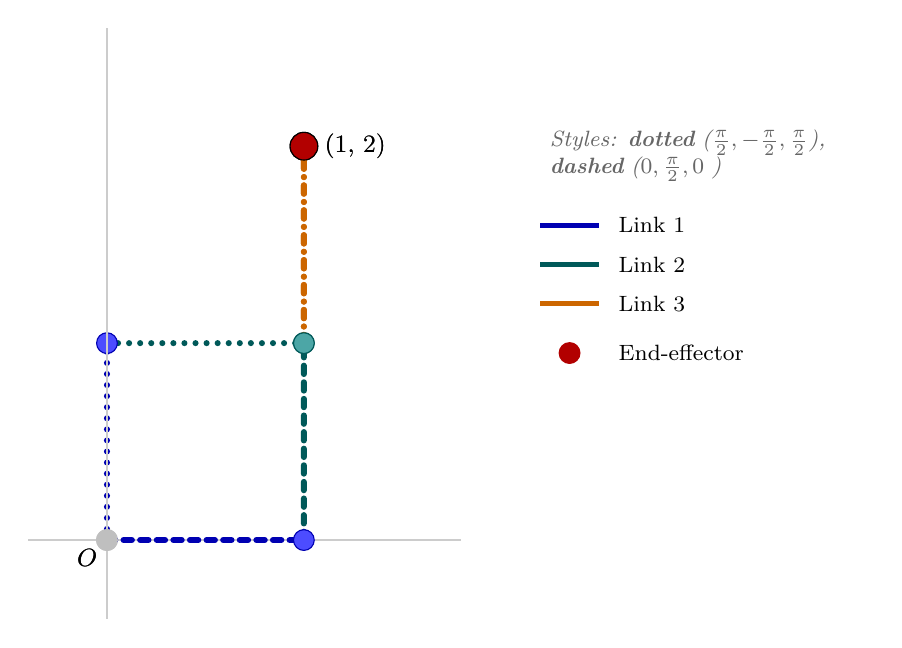
\begin{tikzpicture}[scale=2.5]
  % ── Soluzione 1: theta = [pi/2, -pi/2, pi/2]
  %    cumulative angles: phi1=90, phi2=0, phi3=90
  \begin{scope}[xshift=0cm]
    \drawarm{90}{0}{90}{}{my dotted}
    \drawarm{0}{90}{90}{}{dashed}
  \end{scope}
  % shared legend

  \begin{scope}[xshift=2.2cm, yshift=1.8cm] % Spostata più a destra per dare respiro

    \node[right, font=\footnotesize\itshape, text width=4cm] at (0, 0.15) 
      {\textcolor{black!60}{Styles: \textbf{dotted} ($\frac\pi2, -\frac\pi2, \frac\pi2$), \textbf{dashed} ($0,\frac\pi2,0$ )}};
    
    \foreach \col/\lbl/\y in {
        blue!70!black/Link 1/ -0.2,
        teal!70!black/Link 2/ -0.4,
        orange!80!black/Link 3/ -0.6}{
      \draw[\col, line width=1.8pt] (0,\y) -- (0.3,\y);
      \node[right, font=\footnotesize] at (0.35,\y) {\lbl};
    }
    
    \filldraw[red!70!black] (0.15, -0.85) circle (1.5pt);
    \node[right, font=\footnotesize] at (0.35, -0.85) {End-effector};
  \end{scope}
\end{tikzpicture}
\caption{This picture displays the two solutions (they both reach the point $(1,1)$ but follow two different paths (dotted and dashed), from there they reach point $(1,2)$ (dash dotted) }
\end{figure}

 
\myhrule{}
To implement the methods we follow the formulas 
\begin{align}
    q^{k+1} &= q^k + \alpha J_\kappa^T(q^k) [x_e^d - \kappa(q^k)] \tag{Gradient} \\ 
    q^{k+1} &= q^k + \alpha J_\kappa^{-1}(q^k) [x_e^d - \kappa(q^k)] \tag{Newton}
\end{align}
Then we can use \texttt{sympy} python library to compute the $J_\kappa^{-1}(q^k)$ using the following lines to set up the basic variables:

\begin{lstlisting}[language=Python]
from sympy import sin, cos, Matrix, lambdify
from sympy.abc import alpha, beta,gamma ,kappa
import numpy as np

J = Matrix([ cos(alpha) + cos(alpha+beta) + cos(alpha + beta + gamma) , sin(alpha) + sin(alpha+beta) + sin(alpha + beta + gamma), alpha + beta + gamma])
Y = Matrix([alpha, beta, gamma])
Jac = J.jacobian(Y)
Jinv = Jac**-1 # Inversa
jinv_func = lambdify((alpha, beta, gamma), Jinv, 'numpy')
jac_direct_func= lambdify((alpha, beta, gamma), Jac, 'numpy')
\end{lstlisting}
After that the code follows directly where \texttt{history} is just used for plotting the values and $\alpha,\beta,\gamma$ are used as $\theta_1,\theta_2,\theta_3$.
\begin{lstlisting}[language=Python]
def newton():
    q = np.array(INITIAL, dtype=float) 
    target_pos = np.array(TARGET)
    history=[]
    for i in range(MAX_ITER):
        current_pos = kappa(q=q)
        history.append(current_pos[:2])
        error_vector = target_pos - current_pos    
        if np.linalg.norm(error_vector) < TOL:
            return history    
        inv_j_num = jinv_func(q[0], q[1], q[2])
        q = q + ALPHA * (inv_j_num @ error_vector)   
    return history
\end{lstlisting}

\begin{lstlisting}[language=Python]
def gradient(alpha=ALPHA):
    q = np.array(INITIAL, dtype=float) 
    target_pos = np.array(TARGET)
    history=[]
    for i in range(MAX_ITER):
        current_pos = kappa(q=q)
        history.append(current_pos[:2])
        error_vector = target_pos - current_pos
        
        if np.linalg.norm(error_vector) < TOL:
            return history    
        j_num = jac_direct_func(q[0], q[1], q[2])
        q = q + alpha * (j_num.T @ error_vector)
    return history
\end{lstlisting}


Then, if we plot it: 
\begin{figure}[H]
    \centering
    
\includegraphics[width=0.75\linewidth]{Results/pi-2.png}
    \caption{Results of the two methods with different values of $\alpha$. In this plot we used $q^0=[\frac\pi2,\frac\pi2,\frac\pi2]^\top$. In this configuration, we can see the importance of $\alpha$ since the stepsize actually determines the difference between convergence ($\alpha=0.1$) or bouncing back and forth ($\alpha=0.5$), of course choosing a large stepsize helps in a rapid convergence, but when "close" this could kill the process (indeed, with $\alpha=0.5$ the gradient method does not converge at all even after one million iterations). As done in many deep learning algorithms, a possible choice would be to choose a function for the stepsize $\alpha(n)$ where $n$ is the number of the iteration so that $\alpha(0)$ is regionally big and $\alpha(n)$ being a strictly decreasing function. A small detail that is important to notice is the following: in the top left plot, also the Newton method oscillates between some values so also Newton (for $\alpha=0.5$) does not converge. }
    \label{fig:enter-label}
\end{figure}
The problem arises if $q^0=[0,0,0]^\top$ since it is a singular configuration, in fact: 
$$\det(J) = -\sin(\theta_1)\cos(\theta_1 + \theta_2) + \sin(\theta_1 + \theta_2)\cos(\theta_1) = 2\sin(\theta_2) \quad \footnote{See the code for the calculation using \texttt{sympy}}$$ 
Therefore, Newton's method risks to diverge if not properly adapted to avoid singular configurations. Then, if $\dot q^\star$ is such that $v_e=J\dot q^\star$, also $\dot q = \dot q^\star+P\dot q_0$ is a solution where $P$ is a projection matrix into the null space of $J$ ($\mathcal{N}(J)$) and from algebra we know $P=I-J^\top(JJ^\top)^{-1}J$. We also need to model $\dot q_0 = k_0 \left( \frac{\partial\omega(q)}{\partial q} \right)^\top$ and a typical $\omega$ function used to escaping singularitites is $\omega(q) = \sqrt{\det(J(q) J(q)^\top) +\varepsilon}$ where $\varepsilon\gtrapprox 0$.
Then we need to modify the code listed above, otherwise the solution would be 
\begin{figure}[H]
    \centering
    
\includegraphics[width=0.75\linewidth]{Results/origin.png}
    \caption{Results of the two methods with different values of $\alpha$. In this plot we used $q^0=[0,0,0]^\top$. Again we see the problem of the stepsize $\alpha$.}
    \label{fig:enter-label}
\end{figure}
This proves the issue: we can see that the left plots (the ones of the Newton's method) do not move the robotic arm from its initial position. 

\begin{lstlisting}[language=python]
def redundantNewton(alpha_step=0.1, k0=0.5):
    w_sym = sqrt((Jac.T * Jac).det()+SCALAR_EPSILON) # w = root( det JJ )
    grad_w_sym = w_sym.diff(Y)
    w_func = lambdify((alpha, beta, gamma), w_sym, 'numpy') 
    grad_w_func = lambdify((alpha, beta, gamma), grad_w_sym, 'numpy')
    jac_func = lambdify((alpha, beta, gamma), Jac, 'numpy')
    q = np.array(INITIAL, dtype=float) 
    target_pos = np.array(TARGET)
    history = []

    for i in range(MAX_ITER):
        current_pos = kappa(q=q)
        history.append(current_pos.copy())
        error_vector = target_pos - current_pos    
        if np.linalg.norm(error_vector) < TOL:
            print(f"Target raggiunto {i}")
            return history    
        J_n = jac_func(q[0], q[1], q[2])
        g_w_n = grad_w_func(q[0], q[1], q[2]) 
        J_pinv = np.linalg.pinv(J_n, rcond=1e-3)
        I = np.eye(len(q))
        P = I - J_pinv @ J_n
        q_dot_task = J_pinv @ error_vector
        q_dot_null = P @ (k0 * g_w_n.T).flatten()
        q = q + alpha_step * (q_dot_task + q_dot_null)      
    return history
\end{lstlisting}

We can finally see the results. 

\begin{figure}[H]
    \centering
    
\includegraphics[width=0.75\linewidth]{Results/originWithCorrections.png}
    \caption{Results of the two methods with different values of $\alpha$. In this plot we used $q^0=[0,0,0]^\top$ and the \texttt{redundantNewton} method}
    \label{fig:enter-label}
\end{figure}
A final possible attempt is using the generalized inverse (right pseudo inverse \footnote{Note that in the code below the calculations were done "manually" instead of using the \texttt{pinv} function from \texttt{numpy}}) $J^\dagger=J^\top (J J^\top)^{-1}$ (again we need to be sure that $\det J^\dagger \neq 0$ hence we add $\lambda I$ for $\lambda\gtrapprox 0$). The code is really similar to the previous ones: 

\begin{lstlisting}[language=python]
def generalizedNewton(alpha_step=0.1, lam=0.1):
    q = np.array(INITIAL, dtype=float)
    target_pos = np.array(TARGET)
    history = []
    i=0
    for i in range(MAX_ITER):
        current_pos = kappa(q=q)
        history.append(current_pos[:2].copy())
        error_vector = target_pos - current_pos
        if np.linalg.norm(error_vector) < TOL:
            return history,i
        J_n = jac_direct_func(q[0], q[1], q[2])         
        JJT = J_n @ J_n.T                                   
        J_d = J_n.T @ np.linalg.inv(JJT + lam * np.eye(3))  
        q = q + alpha_step * (J_d @ error_vector)
    return history,i
\end{lstlisting}
The only issue is that computing the pseudo inverse (analytically) takes too much time for \texttt{sympy}, so I had to evaluate it using \texttt{numpy}, which is much faster (but just numerical). 
\begin{figure}[H]
    \centering
    
\includegraphics[width=0.75\linewidth]{Results/Comparison.png}
    \caption{Results of the two methods with different values of $\alpha$. In this plot we used $q^0=[0,0,0]^\top$.}
    \label{fig:enter-label}
\end{figure}
A couple of final considerations can be done: using the two methods on the given inputs, the number of iterations needed for the convergence are:  
\begin{comment}
Start=pi/2, alpha=0.5 -> Generalized: 23 iter | Redundant: 17 iter
Target raggiunto 102 \\ 
Start=pi/2, alpha=0.1 -> Generalized: 151 iter | Redundant: 102 iter
Target raggiunto 20 \\ 
Start=0, alpha=0.5 -> Generalized: 27 iter | Redundant: 20 iter
Target raggiunto 101 \\ 
Start=0, alpha=0.1 -> Generalized: 134 iter | Redundant: 101 iter\\
\end{comment}
\begin{table}[H]
    \centering
    \begin{tabular}{cccc}
        \toprule
        \textbf{Start} & \textbf{Alpha} & \textbf{Generalized } & \textbf{Redundant}  \\
        \midrule
        $\bm{\pi/2}$ & 0.5 & 23 & 17  \\
        $\bm{\pi/2}$ & 0.1 & 151 & 102  \\
        $\bm{0}$       & 0.5 & 27 & 20  \\
        $\bm{0}$       & 0.1 & 134 & 101 \\
        \bottomrule
    \end{tabular}
\end{table}
Overall, the generalized inverse performs worse in terms of the mere number of iterations, it is important to consider that the other path also does not consider other singularities that have to be avoided. 

\myrule{}
\myrule{}






For the second task we can proceed just like the first one: then 
$$\begin{cases}
    \cos(\theta_1) + \cos(\theta_1+\theta_2) + \cos(\theta_1+\theta_2+\theta_3) = 1 \\ 
    \sin(\theta_1) + \sin(\theta_1+\theta_2) + \sin(\theta_1+\theta_2+\theta_3) = 2\\ 
    \theta_1+\theta_2+\theta_3 = -\dfrac{\pi}{2}
\end{cases}$$
The difference is that the $\sin(-\frac\pi 2)$ is $-1$, which means that the second equation becomes
$$\sin(\theta_1) + \sin(\theta_1+\theta_2) + (-1) = 2\\ $$
Hence, the sum of two sines is 3, which is not possible in the real numbers. Then this second configuration is impossible. This was previously calculated in the third case of the analytical solution, so this result comes with no surprise. 


Moreover, I would need to reach the point $(1,3)$ to have an orientation of $-\frac\pi2$ in $(1,2)$, so the minimum overall length of the first two joints should be $\sqrt{10} \approx 3.1622$ and not 2.



\end{document}
